\documentclass[reportComp]{thesis}
\usepackage[python,pseudo]{mypackage}

\title{模式识别作业六}
\school{数据科学与计算机学院}
\author{陈鸿峥}
\classname{17大数据与人工智能}
\stunum{17341015}
\headercontext{模式识别作业作业六}

\begin{document}

\maketitle

\begin{answer}[\textsection 5 Q4]
\begin{itemize}
	\item [(a)] 构造拉格朗日函数
	\[\begin{aligned}f(\mathbf{x}, \lambda)&=\left\|\mathbf{x}-\mathbf{x}_{a}\right\|^{2}+2 \lambda[g(\mathbf{x})]\\
	&=\left\|\mathbf{x}-\mathbf{x}_{a}\right\|^{2}+2 \lambda\left[\mathbf{w}^{t} \mathbf{x}+w_{0}\right] \\
	&=\left(\mathbf{x}-\mathbf{x}_{a}\right)^{t}\left(\mathbf{x}-\mathbf{x}_{a}\right)+2 \lambda\left(\mathbf{w}^{t} \mathbf{x}+w_{0}\right) \\
	&=\mathbf{x}^{t} \mathbf{x}-2 \mathbf{x}^{t} \mathbf{x}_{a}+\mathbf{x}_{a}^{t} \mathbf{x}_{a}+2 \lambda\left(\mathbf{x}^{t} \mathbf{w}+w_{0}\right)
	\end{aligned}\]
	分别求偏导有
	\[\begin{array}{l}
	{\frac{\partial f(\vx, \lambda)}{\partial \vx}=\vx-\vx_{a}+\lambda \vw=0} \\
	{\frac{\partial f(\vx, \lambda)}{\partial \lambda}=\vw^{t} \vx+w_{0}=0}
	\end{array}\]
	联立可解得
	\[\lambda=\frac{\mathbf{w}^{t} \mathbf{x}_{a}+w_{0}}{\mathbf{w}^{t} \mathbf{w}}\]
	进而有
	\[\begin{aligned} \mathbf{x} &=\mathbf{x}_{a}-\lambda \mathbf{w} \\
	&=\left\{\begin{array}{ll}
	{\mathbf{x}_{a}-\left[\frac{\mathbf{w}^{t} \mathbf{x}_{a}+w_{0}}{\mathbf{w}^{t} \mathbf{w}}\right] \mathbf{w}} & {\text { if } \mathbf{w} \neq \mathbf{0}} \\
	{\mathbf{x}_{a}} & {\text { if } \mathbf{w}=\mathbf{0}}
	\end{array}
	\right.\end{aligned}\]
	最终得到距离最小值
	\[\begin{aligned}
	\left\|\mathbf{x}-\mathbf{x}_{a}\right\| &=\left\|\mathbf{x}_{a}-\left[\frac{\mathbf{w}^{t} \mathbf{x}_{a}+w_{0}}{\mathbf{w}^{t} \mathbf{w}}\right] \mathbf{w}-\mathbf{x}_{a}\right\| \\
	&=\left\|\left(\frac{\mathbf{w}^{t} \mathbf{x}_{a}+w_{0}}{\mathbf{w}^{t} \mathbf{w}}\right) \mathbf{w}\right\| \\
	&=\frac{\left|g\left(\mathbf{x}_{a}\right)\right|\|\mathbf{w}\|}{\|\mathbf{w}\|^{2}}=\frac{\left|g\left(\mathbf{x}_{a}\right)\right|}{\|\mathbf{w}\|}
	\end{aligned}\]
	\item [(b)] 由于(a)已经得到从超平面到$\vx$的最小距离,而$\vx_a$的投影即为拉格朗日求导等于零求出来的$\vx$值,即
	\[\begin{aligned}
	\mathbf{x}_{o} &=\mathbf{x}_{a}-\lambda \mathbf{w} \\
	&=\mathbf{x}_{a}-\frac{g\left(\mathbf{x}_{a}\right)}{\|\mathbf{w}\|^{2}} \mathbf{w}
	\end{aligned}\]
	其中
	\[\lambda=\frac{\mathbf{w}^{t} \mathbf{x}_{a}+w_{0}}{\mathbf{w}^{t} \mathbf{w}}=\frac{g\left(\mathbf{x}_{a}\right)}{\|\mathbf{w}\|^{2}}\]
\end{itemize}
\end{answer}

\begin{answer}[\textsection 5 Q14]
将训练集数据$\omega_1$和$\omega_2$构成矩阵,并扩增一个维度,得到
\[\mathbf{Y}=\left(\begin{array}{rrr}{1} & {1} & {5} \\ {1} & {2} & {9} \\ {1} & {-5} & {-3} \\ {-1} & {-2} & {3} \\ {-1} & {1} & {4} \\ {-1} & {0} & {-2}\end{array}\right) \quad \mathbf{a}=\left(\begin{array}{r}{a_{1}} \\ {a_{2}} \\ {a_{3}}\end{array}\right) \quad \mathbf{b}=\left(\begin{array}{c}{b} \\ {b} \\ {b} \\ {b} \\ {b} \\ {b}\end{array}\right)\]
平方误差准则函数为
\[\mathbf{J}_{s}(\mathbf{a})=\frac{1}{2} \sum_{i=1}^{n}\left(\mathbf{a}^{t} \mathbf{y}_{i}-b\right)^{2}=\frac{(\mathbf{Y} \mathbf{a}-\mathbf{b})^{t}(\mathbf{Y} \mathbf{a}-\mathbf{b})}{2}\]
\begin{itemize}
	\item [(a)] 对准则函数求导得到
	\[\nabla J_{s}(\mathbf{a})=Y^{t}(\mathbf{Y} \mathbf{a}-\mathbf{b})=\left(
	\begin{array}{ccccccc}{6 a_{1}} & {-} & {a_{2}} & {+} & {6 a_{3}} & {+} & {0} \\
	{-a_{1}} & {+} & {35 a_{2}} & {+} & {36 a_{3}} & {+} & {3 b} \\
	{6 a_{1}} & {+} & {36 a_{2}} & {+} & {144 a_{3}} & {-} & {16 b}
	\end{array}\right)\]
	进而Hessian矩阵为
	\[\mathbf{H}=\mathbf{Y}^{t} \mathbf{Y}=\left(\begin{array}{ccc}{6} & {-1} & {6} \\ {-1} & {35} & {36} \\ {6} & {36} & {144}\end{array}\right)\]
	\item [(b)] 最优学习率
	\[\eta=\frac{\left[\boldsymbol{\nabla} J_{s}(\mathbf{a})\right]^{t} \boldsymbol{\nabla} J_{s}(\mathbf{a})}{\left[\boldsymbol{\nabla} J_{s}(\mathbf{a})\right]^{t} \mathbf{H} \nabla J_{s}(\mathbf{a})}\]
	通过求解特征方程,得到$\vH$的特征值为$5.417,24.57,155.0$,进而$0.006452\leq\eta\leq 0.1846$
\end{itemize}
\end{answer}

\begin{answer}[\textsection 5 Q21]
由等式(54)有权重向量
\[\mathbf{w}=\alpha n \mathbf{S}_{w}^{-1}\left(\mathbf{m}_{1}-\mathbf{m}_{2}\right)\]
其中$\vw$满足
\[\left[\frac{1}{n} \mathbf{S}_{w}+\frac{n_{1} n_{2}}{n^{2}}\left(\mathbf{m}_{1}-\mathbf{m}_{2}\right)\left(\mathbf{m}_{1}-\mathbf{m}_{2}\right)^{t}\right] \mathbf{w}=\mathbf{m}_{1}-\mathbf{m}_{2}\]

将$\vw$代入得到
\[\left[\frac{1}{n} \mathbf{S}_{w}+\frac{n_{1} n_{2}}{n^{2}}\left(\mathbf{m}_{1}-\mathbf{m}_{2}\right)\left(\mathbf{m}_{1}-\mathbf{m}_{2}\right)^{t}\right] \alpha n \mathbf{S}_{w}^{-1}\left(\mathbf{m}_{1}-\mathbf{m}_{2}\right)=\mathbf{m}_{1}-\mathbf{m}_{2}\]
进而
\[\alpha \theta\left(\mathbf{m}_{1}-\mathbf{m}_{2}\right)=\mathbf{m}_{1}-\mathbf{m}_{2}\]
其中
\[\theta=1+\frac{n_{1} n_{2}}{n^{2}}\left(\mathbf{m}_{1}-\mathbf{m}_{2}\right)^{t} \mathbf{S}_{w}^{-1}\left(\mathbf{m}_{1}-\mathbf{m}_{2}\right)\]
由于这条等式对于所有$\vm_1$和$\vm_2$成立,因此我们有$\alpha\theta=1$,或者下式成立
\[\alpha=\left[1+\frac{n_{1} n_{2}}{n^{2}}\left(\mathbf{m}_{1}-\mathbf{m}_{2}\right)^{t} \mathbf{S}_{w}^{-1}\left(\mathbf{m}_{1}-\mathbf{m}_{2}\right)\right]^{-1}\]
\end{answer}

\begin{answer}[\textsection 5 Q28]
实际上即找
\[\min \left\{t: t \geq 0, \mathbf{a}^{t} \mathbf{y}_{i}+t>b_{i} \text { for all } i\right\}\]
而目标是使权重向量$\va$最小化准则函数
\[J_{t}(\mathbf{a})=\max _{i: \mathbf{a}^{t} \mathbf{y}_{i} \leq b_{i}}\left(b_{i}-\mathbf{a}^{t} \mathbf{y}_{i}\right)\]

将其分为线性可分和线性不可分两种情况处理。
\begin{itemize}
	\item [(a)] 线性可分情况下,存在$\va_o$使得$\va_o^t\vy_i=b_i$,那么显然
	\[\forall t>0,i:\; \va_o^t\vy_i+t > b_i\]
	因此我们有对于所有的$i$
	\[\begin{aligned}
	0 & \leq \min \left\{t: t \geq 0, \mathbf{a}^{t} \mathbf{y}_{i}+t>b_{i}\right\} \\
	 & \leq \min \left\{t: t \geq 0, \mathbf{a}^{t} \mathbf{y}_{i}+t>b_{i}\right\}=0
	\end{aligned}\]
	进而
	\[\min \left\{t: t \geq 0, \mathbf{a}^{t} \mathbf{y}_{i}+t>b_{i}\right\}=0\]
	得到的权重向量即为$\va_o$。
	由$J_t(\va)\geq 0,\forall\va$且$J_t(\va_o)=0$,可知
	\[\arg \min _{\mathbf{a}} J_{t}(\mathbf{a})=\mathbf{a}_{o}\]
	这说明使$\va$最小化$J_t(\va)$等价于解决修改后的问题。
	\item [(b)] 线性不可分下,不存在$\va_o$使得$\va_o^t\vy_i=b_i$,那么
	\[\begin{aligned}
	\forall i:\;\min _{t, \mathbf{a}}\left\{t: t \geq 0, \mathbf{a}^{t} \mathbf{y}_{i}+t>b_{i}\right\}
	&=\min _{t, \mathbf{a}}\left\{t: t \geq 0, t>b_{i}-\mathbf{a}^{t} \mathbf{y}_{i}\right\} \\
	&=\min _{t, \mathbf{a}}\left\{t: t \geq 0, t>\max _{i}\left(b_{i}-\mathbf{a}^{t} \mathbf{y}_{i}\right)\right\} \\
	&=\min _{t, \mathbf{a}}\left\{t: t>0, t>\max _{i}\left(b_{i}-\mathbf{a}^{t} \mathbf{y}_{i}\right)\right\} \\
	&=\min _{t, \mathbf{a}}\left\{t: t>\max _{i: \mathbf{a}^{t} \mathbf{y}_{i} \leq b_{i}}\left(b_{i}-\mathbf{a}^{t} \mathbf{y}_{i}\right)\right\} \\
	&=\min _{t, \mathbf{a}}\left\{\max _{i: \mathbf{a}^{t} \mathbf{y}_{i} \leq b_{i}}\left(b_{i}-\mathbf{a}^{t} \mathbf{y}_{i}\right)\right\} \\
	&=\min _{\mathbf{a}} J_{t}(\mathbf{a})
	\end{aligned}\]
\end{itemize}
\end{answer}

\begin{answer}[\textsection 5 Q32]
\begin{itemize}
	\item [(a)] 按序编号
	\[\begin{aligned}
	\omega_{1}&: \mathrm{x}_{1}=\left(\begin{array}{c}{1} \\ {1}\end{array}\right), \mathrm{x}_{2}=\left(\begin{array}{l}{2} \\ {2}\end{array}\right), \mathrm{x}_{3}=\left(\begin{array}{l}{2} \\ {0}\end{array}\right)\\
	\omega_{2}&:\mathrm{x}_{4}=\left(\begin{array}{l}{0} \\ {0}\end{array}\right), \mathrm{x}_{5}=\left(\begin{array}{l}{1} \\ {0}\end{array}\right), \mathrm{x}_{6}=\left(\begin{array}{l}{0} \\ {1}\end{array}\right)
	\end{aligned}\]
	且$z_1=z_2=z_3=-1,z_4=z_5=z_6=1$。
	最优超平面为$y_1+y_2=3/2$或
	\[(3 / 2,-1,-1)^{t}\left(1,y_{1},y_{2}\right)=0\]
	将其做放缩变换($\times 2$),得到权向量为$(3,-2,-2)^t$。

	\begin{figure}[H]
	\centering
	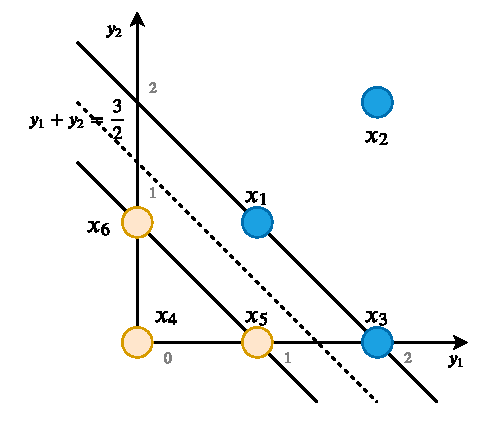
\includegraphics[width=0.5\linewidth]{fig/Q32.pdf}
	\end{figure}
	最优间隔为从样本点到超平面的最小距离,如上图所示,为$\sqrt{2}/4$。
	\item [(b)] 从上图可以清晰看出,支持向量为
	\[\left\{\mathbf{x}_{1}, \mathbf{x}_{3}, \mathbf{x}_{5}, \mathbf{x}_{6}\right\}=\left\{(1,1)^{t},(2,0)^{t},(1,0)^{t},(0,1)^{t}\right\}\]
	\item [(c)] 最大化式(109)给出的准则函数
	\[\begin{aligned}
	& L(\boldsymbol{\alpha})=\sum_{k=1}^{n} \alpha_{k}-\frac{1}{2} \sum_{k, j}^{n} \alpha_{k} \alpha_{j} z_{k} z_{j} \mathbf{y}_{j}^{t} \mathbf{y}_{k}\\
	& \text{s.t.} \sum_{k=1}^{n} z_{k} \alpha_{k}=0,\;\alpha_k\geq 0
	\end{aligned}\]
	使用约束条件,可用下式消除一个元
	\[\alpha_{6}=\alpha_{1}+\alpha_{2}+\alpha_{3}-\alpha_{4}-\alpha_{5}\]
	求偏导得到
	\[\left[\begin{array}{ccccc}{-1} & {-2} & {-2} & {0} & {1} \\ {-2} & {-5} & {2} & {-1} & {1} \\ {-2} & {2} & {-5} & {1} & {1} \\ {0} & {-1} & {1} & {-1} & {-1} \\ {1} & {1} & {3} & {-1} & {-2}\end{array}\right]\left[\begin{array}{c}{\alpha_{1}} \\ {\alpha_{2}} \\ {\alpha_{3}} \\ {\alpha_{4}} \\ {\alpha_{5}}\end{array}\right]=\left[\begin{array}{c}{-2} \\ {-2} \\ {-2} \\ {0} \\ {0}\end{array}\right]\]
	但是这个方程组不相容,因此最大值一定在边界处取到(即有些$\alpha_i$消失了)。
	接下来尝试分别令每一个$\alpha_i=0$来求解。
	\begin{itemize}
	\item $\alpha_1=0$时,
	\[\frac{\partial L\left(0, \alpha_{2}, \alpha_{3}, \alpha_{4}, \alpha_{5}\right)}{\partial \alpha_{i}}=0\]
	可解得$\boldsymbol{\alpha}=(0,-1/10,-1/10,8/5,-8/5,-4/5)^{t}$
	\item $\alpha_2=0$时,下式导致不相容
	\[\frac{\partial L\left(\alpha_{1}, 0, \alpha_{3}, \alpha_{4}, \alpha_{5}\right)}{\partial \alpha_{i}}=0\]
	\item $\alpha_3=0$时,下式导致不相容
	\[\frac{\partial L\left(\alpha_{1}, \alpha_{2}, 0, \alpha_{4}, \alpha_{5}\right)}{\partial \alpha_{i}}=0\]
	\item $\alpha_4=0$时,
	\[\frac{\partial L\left(\alpha_{1}, \alpha_{2}, \alpha_{3}, 0, \alpha_{5}\right)}{\partial \alpha_{i}}=0\]
	解得$\boldsymbol{\alpha}=1/5(16,0,4,0,14,6)^{t}$,满足$\alpha_i\geq 0$的限制,此时准则函数$L(\valpha)=4$
	\item $\alpha_5=0$时,
	\[\frac{\partial L\left(\alpha_{1}, \alpha_{2}, \alpha_{3}, \alpha_{4}, 0\right)}{\partial \alpha_{i}}=0\]
	得到$\valpha=1 / 5(2,2,2,0,0,6)^{t}$,满足$\alpha_i\geq 0$的限制,此时准则函数$L(\valpha)=1.2$
	\end{itemize}
	故$\boldsymbol{\alpha}=1/5(16,0,4,0,14,6)^{t}$时,准则函数$L$取得最大值,且满足限制条件。

	接下来计算权向量$\va$。
	视$\va$为变量,尝试最小化式(108)中的
	\[L(\mathbf{a}, \boldsymbol{\alpha})=\frac{1}{2}\|\mathbf{a}\|^{2}-\sum_{k=1}^{n} \alpha_{k}\left[z_{k} \mathbf{a}^{t} \mathbf{y}_{k}-1\right]\]
	求导有
	\[\frac{\partial L}{\partial \mathbf{a}}=\mathbf{a}-\sum_{k=1}^{n} \alpha_{k} z_{k} \mathbf{y}_{k}=\mathbf{0}\]
	进而$\va=(0,-2,-2)^t$。

	最后确定$a_0$。
	使用支持向量$\vy=(1,1,1)^t$,满足$\va^t\vy_1z_1=1$,得到
	\[-\left(\begin{array}{c}{0} \\ {-2} \\ {-2}\end{array}\right)(1,1,1)=-a_{0}+4=1\]
	故$a_0=3$,最终的权向量为$\va=(3,-2,-2)^t$。
\end{itemize}
\end{answer}

\end{document}